%% BioMed_Central_Tex_Template_v1.06
%%                                      %
%  bmc_article.tex            ver: 1.06 %
%                                       %

%%IMPORTANT: do not delete the first line of this template
%%It must be present to enable the BMC Submission system to
%%recognise this template!!

%%%%%%%%%%%%%%%%%%%%%%%%%%%%%%%%%%%%%%%%%
%%                                     %%
%%  LaTeX template for BioMed Central  %%
%%     journal article submissions     %%
%%                                     %%
%%          <8 June 2012>              %%
%%                                     %%
%%                                     %%
%%%%%%%%%%%%%%%%%%%%%%%%%%%%%%%%%%%%%%%%%


%%%%%%%%%%%%%%%%%%%%%%%%%%%%%%%%%%%%%%%%%%%%%%%%%%%%%%%%%%%%%%%%%%%%%
%%                                                                 %%
%% For instructions on how to fill out this Tex template           %%
%% document please refer to Readme.html and the instructions for   %%
%% authors page on the biomed central website                      %%
%% http://www.biomedcentral.com/info/authors/                      %%
%%                                                                 %%
%% Please do not use \input{...} to include other tex files.       %%
%% Submit your LaTeX manuscript as one .tex document.              %%
%%                                                                 %%
%% All additional figures and files should be attached             %%
%% separately and not embedded in the \TeX\ document itself.       %%
%%                                                                 %%
%% BioMed Central currently use the MikTex distribution of         %%
%% TeX for Windows) of TeX and LaTeX.  This is available from      %%
%% http://www.miktex.org                                           %%
%%                                                                 %%
%%%%%%%%%%%%%%%%%%%%%%%%%%%%%%%%%%%%%%%%%%%%%%%%%%%%%%%%%%%%%%%%%%%%%

%%% additional documentclass options:
%  [doublespacing]
%  [linenumbers]   - put the line numbers on margins

%%% loading packages, author definitions

\documentclass[twocolumn]{bmcart}% uncomment this for twocolumn layout and comment line below
%\documentclass{bmcart}

%%% Load packages
%\usepackage{amsthm,amsmath}
%\RequirePackage{natbib}
%\RequirePackage[authoryear]{natbib}% uncomment this for author-year bibliography
%\RequirePackage{hyperref}
\usepackage[utf8]{inputenc} %unicode support
\usepackage{graphicx}
\usepackage{float}
\restylefloat{figure}
\usepackage[export]{adjustbox}
\usepackage{caption}
\renewcommand{\figurename}{Fig}
%\usepackage[applemac]{inputenc} %applemac support if unicode package fails
%\usepackage[latin1]{inputenc} %UNIX support if unicode package fails


%%%%%%%%%%%%%%%%%%%%%%%%%%%%%%%%%%%%%%%%%%%%%%%%%
%%                                             %%
%%  If you wish to display your graphics for   %%
%%  your own use using includegraphic or       %%
%%  includegraphics, then comment out the      %%
%%  following two lines of code.               %%
%%  NB: These line *must* be included when     %%
%%  submitting to BMC.                         %%
%%  All figure files must be submitted as      %%
%%  separate graphics through the BMC          %%
%%  submission process, not included in the    %%
%%  submitted article.                         %%
%%                                             %%
%%%%%%%%%%%%%%%%%%%%%%%%%%%%%%%%%%%%%%%%%%%%%%%%%


%\def\includegraphic{}
%\def\includegraphics{}




%%% Put your definitions there:
\startlocaldefs
\endlocaldefs


%%% Begin ...
\begin{document}

%%% Start of article front matter
\begin{frontmatter}

\begin{fmbox}
\dochead{Machine Learning and Swarm Intelligence}

%%%%%%%%%%%%%%%%%%%%%%%%%%%%%%%%%%%%%%%%%%%%%%
%%                                          %%
%% Literature Review of Machine Learning Applied to Swarm Robotics     %%
%%                                          %%
%%%%%%%%%%%%%%%%%%%%%%%%%%%%%%%%%%%%%%%%%%%%%%


\title{Machine Learning and Swarm Intelligence Coming Together: A Literature Review  }

%%%%%%%%%%%%%%%%%%%%%%%%%%%%%%%%%%%%%%%%%%%%%%
%%                                          %%
%% Enter the authors here                   %%
%%                                          %%
%% Specify information, if available,       %%
%% in the form:                             %%
%%   <key>={<id1>,<id2>}                    %%
%%   <key>=                                 %%
%% Comment or delete the keys which are     %%
%% not used. Repeat \author command as much %%
%% as required.                             %%
%%                                          %%
%%%%%%%%%%%%%%%%%%%%%%%%%%%%%%%%%%%%%%%%%%%%%%
%\author[
%   addressref={aff1},                   % id's of addresses, %e.g. {aff1,aff2}
%   corref={aff1},                       % id of corresponding %address, if any
%   noteref={n1},                        % id's of article %notes, if any
%   email={dsibrahim@mun.ca}   % email address
%]{\inits{DI}\fnm{Dalia} \snm{Ibrahim}}

\author[
   addressref={aff1},
   email={cdsalcedo@mun.ca}
]{\inits{CD}\fnm{Carlos D} \snm{Salcedo}}

\author[
   addressref={aff1},                   % id's of addresses, 
   email={dsibrahim@mun.ca}   % email address
]{\inits{DI}\fnm{Dalia} \snm{Ibrahim}}

\address[id=aff1]{%                           % unique id
  \orgname{Memorial University of Newfoundland}, % university, etc
  \street{230 Elizabeth Ave},                     %
  \postcode{A1C 5S7}                                % post or zip code
  \city{St. John's},                              % city
  \cny{Canada}                                    % country
}

%%%%%%%%%%%%%%%%%%%%%%%%%%%%%%%%%%%%%%%%%%%%%%
%%                                          %%
%% Enter short notes here                   %%
%%                                          %%
%% Short notes will be after addresses      %%
%% on first page.                           %%
%%                                          %%
%%%%%%%%%%%%%%%%%%%%%%%%%%%%%%%%%%%%%%%%%%%%%%

\begin{artnotes}
%\note{Sample of title note}     % note to the article
%\note[id=aff2]{Equal contributor} % note, connected to author
\end{artnotes}

%\end{fmbox}% comment this for two column layout

%%%%%%%%%%%%%%%%%%%%%%%%%%%%%%%%%%%%%%%%%%%%%%
%%                                          %%
%% The Abstract begins here                 %%
%%                                          %%
%% Please refer to the Instructions for     %%
%% authors on http://www.biomedcentral.com  %%
%% and include the section headings         %%
%% accordingly for your article type.       %%
%%                                          %%
%%%%%%%%%%%%%%%%%%%%%%%%%%%%%%%%%%%%%%%%%%%%%%

\begin{abstractbox}

\begin{abstract} % abstract

Machine learning (ML) and swarm robotics (SR) have been interesting areas of research in the academic and scientific world for decades. Although ML and SR may be considered to be two different types of artificial intelligence (AI), they are not mutually exclusive and there are  multiple applications in the literature where these technologies coincide. This paper discusses the two fields and their relationships by providing examples of the work and research conducted in each of these areas. Three distinct manners in which ML and SR interact with each other are discussed in this paper. The first refers to how scientists are using Swarm Intelligence (SI) and ML in separate tasks to achieve a specific goal, e.g. using SR to gather data, and then using ML to make use of the gathered data. ML and SI also have the potential to make each other better. Therefore, another way consist of ML algorithms applied to SR to optimize the behavior of the swarms and improve their efficiency in specific tasks. The third manner focuses on some of the SI methods that are being used in ML algorithms in an effort to obtain better ML models. 

%\parttitle{First part title} %if any
%Text for this section.
%\parttitle{Second part title} %if any
%Text for this section.
\end{abstract}

%%%%%%%%%%%%%%%%%%%%%%%%%%%%%%%%%%%%%%%%%%%%%%
%%                                          %%
%% The keywords begin here                  %%
%%                                          %%
%% Put each keyword in separate \kwd{}.     %%
%%                                          %%
%%%%%%%%%%%%%%%%%%%%%%%%%%%%%%%%%%%%%%%%%%%%%%

\begin{keyword}
\kwd{Swarm Robotics}
\kwd{Swarm Intelligence}
\kwd{Machine Learning}
\end{keyword}

% MSC classifications codes, if any
%\begin{keyword}[class=AMS]
%\kwd[Primary ]{}
%\kwd{}
%\kwd[; secondary ]{}
%\end{keyword}

\end{abstractbox}
%
\end{fmbox}% uncomment this for twcolumn layout

\end{frontmatter}

%%%%%%%%%%%%%%%%%%%%%%%%% start of article main body
% <put your article body there>

\section*{Introduction}
Machine Learning (ML) and Swarm Intelligence (SI) are arguably two of the most powerful and revolutionary technologies of the twenty first century. As such, many scientists have begun combining or applying both technologies to give rise to more efficient algorithms or better ways of solving real-world problems. However, as mentioned in \cite{James}, depending on what the desired outcome might be, multiple algorithms and techniques need to be tried and tested before a final decision can be made. In other words, selecting the most appropriate algorithms for a given task needs to be done on a per-scenario basis, rather than simply assuming that one method will always perform better than another one. For this reason, this article discusses various ways in which researchers are combining and applying ML and SI in an effort to find better solutions and algorithms. There are three distinct cases in which SI and ML are used together: using SI and ML for separate tasks to accomplish a specific goal, using SI to optimize ML models, and using ML methods to improve the behavior of Swarm Robotics (SR) and SI algorithms. 

\section*{History of Swarm Robotics}
Swarm robotics has been a popular topic in science fiction and the entertainment industry for years, but making such technology a reality is not a particularly easy task. Swarm robotics, as a field of research, is the study of how multiple autonomous robots can be used to accomplish collective tasks that would otherwise be impossible or highly impractical to achieve if they were done by a single robot \cite{Bayindir}. A search of the keywords "swarm robotics" yields over 1,500 results on IEEE Xplore database alone, and there are plenty of projects in the field, such as RoboCup, COLLMOT, Kilobot and TERMES, that show how popular this subject is in the scientific community \cite{Vehlken, Mohan}. According to professor Magnus Egerstedt, it is "annoying" to get a single robot to perform a single task, so getting a bunch of robots to do anything is an impressive achievement on its own \cite{TEDx}. However, to understand swarm robotics, it is important to understand the concept of swarm intelligence (SI). SI refers to the principles that seem to generate the behavior that arises in the interactions between the individual members of the system \cite{Bayindir, Mohan, Webb, Couceiro2014}.

Most of the algorithms behind SI are actually based on the behaviors of ant colonies, schools of fish, flocks of birds, bees, and many other fields where swarms occur \cite{Nedjah}. As an example, ants and termites are able to indirectly communicate with each other. They do not congregate and decide on the schematics of their hives, or how they are going to build them; they just start building without knowing what the other ants are doing \cite{TEDx, TEDx2016}. Scientists use the word stigmergy to describe this phenomenon,  which is a term that refers to the idea that individuals communicate through changes in the world, rather than directly with each other. As each individual modifies a small part of its environment, other members react to this modification and somehow know what to do next.  \cite{TEDx2016, SHoR} 

Significant research in swarm robotics can be found in papers as far back as the 1980s, and the vast theoretical applications of SR have since lead to a great increase of the research in the area \cite{Parker}. However, it is only in the past two decades that theoretical research has started to take form in the physical world, as computational requirements are finally starting to be met. Additionally, the price for the construction of simple robots has decrease dramatically compared to the 1980s and 1990s \cite{Bayindir, Mohan}. Bakhshipour et al. briefly describe over twenty-five heuristic algorithms that could be used for SR search tasks in a single table: one from 1975, four from the 1980s and 1990s, and twenty algorithms from 2005 to 2015 alone. This hints at how many more advancements in the field have occurred in the twenty first century \cite{Bakhshipour}.

In a general sense, the literature indicates that any given SR system must have all of the following characteristics \cite{TEDx, Brambilla}: 
\begin{enumerate}
  \item Robots are completely autonomous: there is no need for direct human interaction or a centralized or universal controller
  \item Robots are safe and reactive
  \begin{itemize}
     \item Capable of adapting to their environment
     \item Able to continue their individual tasks regardless of the number of other robots added or removed
   \end{itemize}
  \item Robot sensing and communication is local, as global knowledge may not be available to any of the bots
  \item Robots cooperate to achieve a given task 
\end{enumerate} 

Some of the main challenges for the adoption of robots in mass scale are large areas to cover, highly dynamic terrains, and constantly changing environments \cite{Couceiro}. However, the characteristics of SR may offer a solution to many of these problems, as adaptability and the ability to cooperate with others are essentially the same characteristics that have allowed humans to be successful in multiple areas \cite{Henrich}. 

\section*{The Basics of Machine Learning}
ML is considered to be a branch of artificial intelligence, but it is actually a multidisciplinary field that makes use of probability and statistics, computational complexity theory, information theory, neurobiology, control theory, philosophy, psychology, and  many other fields. Professor T.M. Mitchell explains, "A computer program is said to learn from experience E with respect to some class of tasks T and performance measure P, if its performance at tasks in T, as measured by P, improves with experience E" \cite{Mitchell}. Ultimately, the purpose of machine learning is to program computers to optimize their performance for a certain task using example data or past experience \cite{Alpaydin}.  As a quick summary of the history of ML, one can take a look into the following historic highlights: the beginning in 1943 with the introduction of the first neural network, contributions from Alan Turing in the 1950s, the creation of Eliza and ALPAC in the 1960s, a shift in research towards knowledge based systems in the 1970s, the discovery of back-propagation and the application of neural networks in new domains in the 1980s, IBM's Deep Blue in the 1990s, and IBM's Watson in the 2000s. Current research in the area focuses on natural language processing, image processing, computer vision, hearing, pattern recognition, and more \cite{Mohammed}. 

Since ML includes a large number of topics, it has been divided into four categories: supervised learning, unsupervised learning, semi-supervised learning, and reinforcement learning. Fig. 1 provides a more detailed description of these categories \cite{Mohammed}. Most of the ML algorithms applied to SR found during the making of this paper were in the area of reinforcement learning (RL) and neural networks, which is not surprising as these methods have become a popular trend in AI during recent years \cite{Corea}. RL is a trial and error method in which an agent learns by interacting with its environment and obtaining a reward or penalty depending on its actions \cite{Iima2}. NN, on the other hand, are a type of non-linear statistical model inspired by the human brain \cite{Hastie}. 

\begin{figure}[H]
 \begin{center} 
  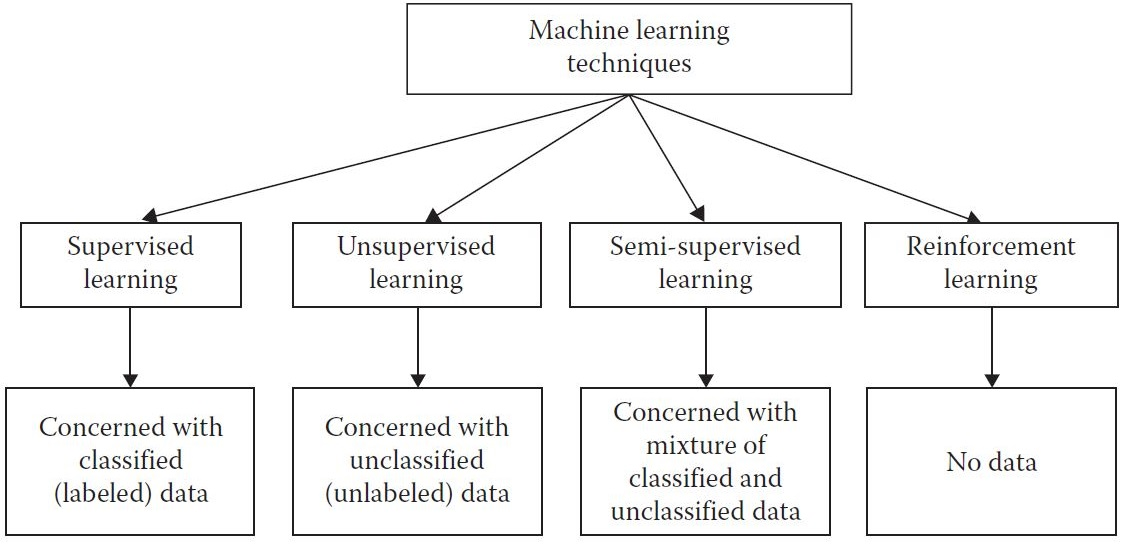
\includegraphics[width=\linewidth]{Types_of_ML.jpg}
  \caption{Imaged obtained from \cite{Mohammed}, which describes the four ML algorithms, and the type of data it requires.}
  \end{center}
\end{figure}


\section*{SI and ML: Separate Tasks, One Objective}

Robots are generally built for the "three D's": dangerous, dirty, and dull tasks, but SR allows robots to also work on a fourth D: distributed tasks \cite{CHF}. This additional D makes SR ideal for gathering data from nearly any physical space, from hard-to-reach places to wide open areas. However, data itself is useless unless valuable information can be gathered from it \cite{Welling}. Fortunately, data is considered by many to be the foundation of ML \cite{Corea, Sundblad}, meaning that the information obtained from SR can potentially be used to train ML models and provide real-world value. One of the most popular examples of this can be found in \cite{Kumar2019}, specifically in the precision farming project, where swarm drones and NN are used to analyze the health of a plantation and estimate its crop yields \cite{TED,AMNH}. For this project, the researchers trained a Fully Convolutional Neural Network (FCN) to detect the apples or oranges in the video footage gathered from the drones, which is ultimately used to determine the amount of fruit in the plantation. Possible directions of future work for this project include testing on other types of trees and plantations and estimation of the average physical size of the fruit \cite{Kumar2018}. Although the authors do not mention possible uses of their project for other areas, one could easily theorize that the ability to count and track objects over video footage, and from multiple sources like the swarm drones, should also be useful for other applications. As an example, their project could probably be used for counting the amount of people in a given area (i.e. stadiums and riots), items in warehouse or store, cars in a parking lot, etc.  An image extracted from \cite{Kumar2018} has been added in the appendix section which further explains the complete process of the fruit classification and counting. 

Another interesting example is found in \cite{Iima}, where the objective is to make a group of robots form a certain shape. Although the task may sound simple, dealing with multiple robots, complicated shapes, and collisions, make it nearly impossible for any person to code every possible combination and scenario imaginable. To solve this issue, the researches in \cite{Iima} implemented a mixture of RL and SI intelligence methods, to find the best policy for the robots to reach multiple predefined formations. Each robot used a Q-Learning algorithm, a type of RL, designed to help the robots find the optimal way of achieving the formation. Since there are multiple robots, the researchers used three policies for updating the robots' Q-Tables: Best, Average, and Particle Swarm Optimization(PSO). The combination of Q-Learning and the SI methods applied for updating the Q-tables proved to be an efficient solution to the robot formation problem.  


\section*{ML to Improve SR}

Human intelligence, which embraces individual, social, and collective wisdom, is the inspiration and foundation for artificial intelligence \cite{Zheng2017}. SI can be considered an attempt at utilizing the social and collective wisdom of individual agents to tackle problems, but the algorithms in SI are not always as efficient as they should be. To help SI solve this problem, several ML methods and algorithms are being applied to existing SI systems. For instance, one of the biggest challenges in SR, is solving the problem of scalability and interchangeability when a large number of robots are involved. In a way, a significant number of popular methods become virtually useless when the number of robots increases dramatically. One of the main reasons this happens is that as the number of robots increases, the computational complexity increases to the point where the system is unable to cope with all the information being shared by the agents. This can also be a problem for some NN, as they are usually unable to deal with inputs of different sizes \cite{Max}. As a way to solve this issue, a combination of various ML methods, primarily those in reinforcement learning (RL), are necessary if scientist hope to find truly scalable and suitable algorithms for multi-agent systems like SR \cite{Lowe}.

A promising example can be found in \cite{Max2}, where deep RL is used for the rendezvous and pursuit evasion problems in SI tasks. To compensate for the previously mentioned problems, the researchers use mean embeddings inspired from the kernel Hilbert spaces. By using mean embeddings, the agents do not need to process all of the information from their neighbors, and instead, learn from a global average. This is a particularly interesting paper as it combines NN, RL, and SI \cite{Max}. Although this experiment was only done on computer simulations, it is plausible to see these algorithms being implemented in the future to get drones and autonomous vehicles to efficiently meet up in a given destination (rendezvous) or even for police pursuits. Other popular examples of ML in SR can be found in \cite{Amigo}, but more updated information can be found online at \cite{RoboCup}. Finally, it is worth mentioning that there are plenty of platforms designed for multi-agent environment simulations like MAgent, OpenAI Gym/Universe, ALE, Malmo, and SC2LE \cite{Zheng2017}.

\section*{SI to Improve ML}

New advancements in SR to help humanity are constantly being researched, like in \cite{Penders}, \cite{Murphy}, \cite{Lomonaco} and \cite{Wilson}, and in many cases, some of these advancements also come with the benefit of being useful in other areas of research. Such has been the case of a multitude of SI algorithms, like Particle Swarm Optimization (PSO) \cite{Bakhshipour, Han} and Ant Colony Optimization (ACO) \cite{Zhiguo2}, both of which are currently being used to improve multiple ML applications. To obtain effective ML systems, several features, configurations, and other factors need to be tweaked, which ultimately ends up leading to extensive testing and monitoring requirements \cite{Breck}. Additionally, some of the popular optimization functions in ML like Stochastic Gradient Descent (SGD) suffer from certain drawbacks like the stopping criteria, learning rate, learning epochs, and local minima \cite{Han}. SI can help alleviate some of these problems by trying multiple options simultaneously and determining the best course of action based on the obtained results. In other words, SI is capable of yielding better results, not because it tries multiple options at the same time, but because SI also includes methods for analyzing, sharing, and communicating the various results obtained and providing a sort of consensus as to in which direction each of the models should go. 

A lot of the uses of SI in ML generally involve PSO or a variation of it. In PSO, there are three vectors, or variables, that each particle takes into account before deciding which way to go: global best (GB), individual best (IB), and a random vector (RV). Depending on the research project, the variables for the vectors and the particles may be defined differently, but the idea remains the same. For example, a particle can easily be a swarm robot, a ML process, an agent, etc. Regarding the variables, GB stands for global best, and it refers to the best position found by the swarm so far. IB is individual best, and it refers to best position that a particle has seen as it moves through space. Finally, RV is a random vector which allows for the particle to randomly explore as it moves to the best position. If particle P, for example, finds a position better than the current GB, the GB will be updated for the entire swarm, and all particles will now start moving towards the position found by P. All the particles in the swarm will move towards their respective IB and RV, and towards the GB, eventually converging in a single point. Using PSO as the optimization function for certain ML algorithms actually avoids some of the drawbacks present in other traditional methods \cite{Kennedy, PSO}. Some popular examples of PSO have been presented in Extreme Learning Machines (ELM), which are a type of single-hidden-layer feedforward neural networks (SLFNs) \cite{Zeng}. In \cite{Han}, the researches showed that using PSO in ELMs resulted in better generalization performance and suggested the idea of using their algorithm in the future for more complex areas, such as gene expression. Since PSO is capable of simultaneously exploring a wider area of the parameter space than other methods like SGD, it would not be surprising to see PSO and variations of it in more NN related research areas.

Another popular SI method used in ML is ACO, which is inspired by the pheromone trails that ants leave behind as they move through their environment. When ants want to move between their colony, C, and some food source, F, they will start randomly moving through multiple paths. If the shortest path is P, then ants moving through P will travel more frequently between C and F. Since ants are passing more often through P, the pheromone scent on P will become stronger than that of the other paths. Eventually, more and more ants will start perceiving that P has a stronger scent and decide to follow P instead of the other paths \cite{Dorigo}. ACO has even been shown to be able to solve the traveling salesman problem. As a simple example, an improved Q-Learning algorithm using ACO was proposed by \cite{Zhiguo}, where the researchers compared their algorithm versus the standard Q-Learning for a maze solving task with multiple robots. ACO showed improvement over the standard Q-Learning algorithm solving the maze in 138 seconds versus 153 seconds with Q-Learning alone. 

\section*{Conclusion}
SI and ML are ideal partners for real-world applications, as they are capable of complementing each other in powerful ways. SI methods may allow ML models to explore new optimization techniques, reduce training times, and find better solutions. On the other hand, ML methods have the possibility of helping swarm robots to find more optimal policies and achieve a higher level of team work. And even when these technologies are not influencing each other directly, they can be utilized together to form pipelines that provide an added value not found  anywhere else. Overall, SI and ML are powerful technologies that will continue to grow in popularity over the coming years and change people's lives for the better.  

\begin{backmatter}

\section*{Acknowledgements}
We would like to thank Memorial University, specially Dr. Lourdes Peña-Castillo, for her support, guidance, and patience during the semester.  





%\bibliographystyle{ieeetr} % Style BST file (bmc-mathphys, vancouver, spbasic).
\bibliography{bmc_article}
\bibliographystyle{bmc-mathphys} % Style BST file (bmc-mathphys, vancouver, spbasic).

\pagebreak
\onecolumn
\section*{Appendix}
%  \begin{figure}[H]
%  \includegraphics[scale=.25]{./Types\_of\_ML.JPG}
%       \caption{\csentence{Sample figure title.}
%      A short description of the figure content
%     should go here.}
%     \end{figure}

\begin{figure}[H]
 \begin{center} 
  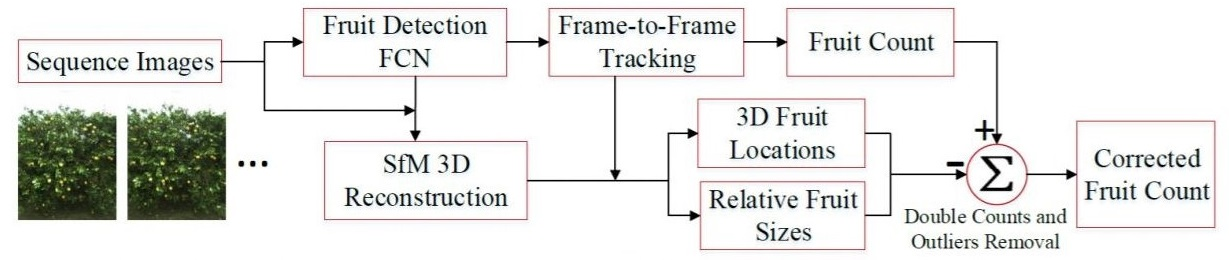
\includegraphics[width=\textwidth]{Kumar2019_crop_yields2.JPG}
  \caption{Image copied directly from \cite{Kumar2018}. A formal description in the authors' own words, "Our fruit counting pipeline consists of detection, tracking, and 3D localization stages. The segmentation stage uses an FCN to segment image into fruit and non-fruit pixels. The tracking stage then tracks the fruits based on the FCN outputs. The 3D localization stage uses SfM reconstruction to estimate fruit 3D locations and size. Finally, based on these localization and size estimation results, we correct the total fruit count from tracking stage, and obtain the corrected fruit count" \cite{Kumar2018}.}
  \end{center}
\end{figure}



\end{backmatter}
\end{document}
